% !TEX root =  ../main_manuscript.tex 
\section{Personalized Schedule of Invasive Tests for Detecting Progression} 
\label{sec:schedule}

\subsection{Cumulative-risk of progression} 
\label{subsec:cum_risk}
Using the joint model fitted to the training data $\mathcal{A}_n$, we aim to derive a personalized schedule of invasive tests for a new patient $j$ with true progression time $T^*_j$. The basis of our calculations is the dynamic cumulative-risk function. Let $t < T^*_j$ be the time of the last conducted test on which progression was not observed. Let $\{\mathcal{Y}_{1j}(v), \ldots, \mathcal{Y}_{Kj}(v)\}$ denote the history of observed longitudinal data up to the current visit time $v$. The current visit can be after the last negative test, i.e., $v \geq t$ (e.g., PSA after negative biopsy in prostate cancer). The cumulative-risk of progression for patient $j$ at future time $u$ is then defined as:
\begin{eqnarray}
\label{eq:cumulative_risk}
\nonumber \lefteqn{R_j(u \mid t, v) = \mbox{Pr}\big\{T^*_j \leq u \mid T^*_j > t, \mathcal{Y}_{1j}(v), \ldots, \mathcal{Y}_{Kj}(v), \mathcal{A}_n\big\}}\\
\nonumber & = & \int \int \mbox{Pr}(T^*_j \leq u \mid T^*_j > t, \boldsymbol{b}_{j}, \boldsymbol{\theta}) \; p\big\{\boldsymbol{b}_j \mid T^*_j > t, \mathcal{Y}_{1j}(v), \ldots, \mathcal{Y}_{Kj}(v), \boldsymbol{\theta} \big\}\\
& & \quad \quad \times \; p(\boldsymbol{\theta} \mid \mathcal{A}_n) \; \mathrm{d}\boldsymbol{b}_j \mathrm{d}\boldsymbol{\theta}, \quad u \geq t,
\end{eqnarray}
The cumulative-risk function $R_j(\cdot)$ dynamically updates over time as more longitudinal data becomes available (Panel~B~and~C, Figure~\ref{fig:dynrisk_explanation}).
\begin{figure}
\centerline{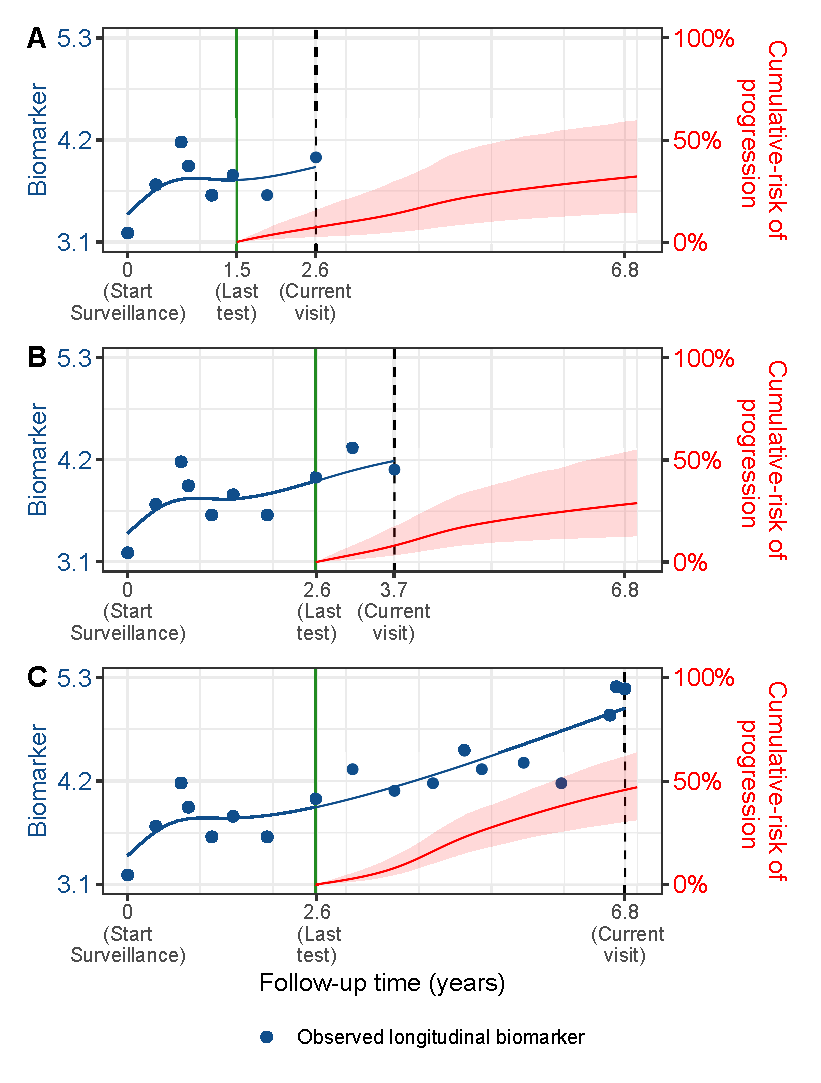
\includegraphics{images/dynrisk_plot_102.eps}}
\caption{\textbf{Cumulative-risk of progression updated dynamically over follow-up} as more patient data is gathered. A single longitudinal outcome, namely, a continuous biomarker of disease progression, is used for illustration. \textbf{Panels~A,~B~and~C:} are ordered by the time of the current visit (dashed vertical black line) of a new patient. At each of these visits, we combine the accumulated longitudinal measurements (shown in blue), and last time of negative invasive test (solid vertical green line) to obtain the updated cumulative-risk profile (shown in red) of the patient. All values are illustrative.} 
\label{fig:dynrisk_explanation}
\end{figure}

\subsection{Personalized Decision Rule} 
\label{subsec:pers_schedule}
We intend to exploit the cumulative-risk function $R_j(\cdot)$ to develop a risk-based personalized schedule of invasive tests for the $j$-th patient. Typically, invasive procedures are decided on the same visit times on which longitudinal data (e.g., biomarkers) are measured. Let $U = \{u_1, \ldots, u_L\}$ represent a schedule of such visits (e.g., biannual PSA measurement in prostate cancer), where $u_1 = v$ is also the current visit time. The last time $u_L$ is selected on the basis of the available information in the original dataset $\mathcal A_n$. That is, tests for the new patient $j$ are planned only up to a future visit time $u_L$ at which sufficient number of events in $\mathcal A_n$ are available (e.g., up to the 80\% or 90\% percentile of progression times). 

We propose conducting a test at a future visit time $u_l \in U$ if the cumulative-risk of progression at $u_l$ exceeds a certain \textit{threshold} $\kappa$ (e.g., 10\% risk). The test decision is given by:
\begin{equation}
\label{eq:personalized_decision_grid}
Q_j^\kappa (u_l \mid t_l, v) = I \big \{ R_j(u_l \mid t_l, v) \geq \kappa \big\}, \quad 0 \leq \kappa \leq 1,
\end{equation}
where $I(\cdot)$ is the indicator function, and $t_l < u_l$ is the time of the last test conducted before the current decision time $u_l$. If a test is planned at $u_l$, then $t_{l+1}=u_l$ becomes the last test time for the next decision time $u_{l+1}$. Otherwise $t_{l+1}$ remains same as $t_l$. Specifically:
\begin{equation*}
t_l = \left \{ 
\begin{array}{ll}
t, & \mbox{if } l = 1\\
t_{l-1}, & \mbox{if } l \geq 2 \mbox{ and } Q_j^\kappa (u_{l-1} \mid t_{l-1}, v) = 0\\
u_{l-1}, & \mbox{if } l \geq 2 \mbox{ and } Q_j^\kappa (u_{l-1} \mid t_{l-1}, v) = 1\\
\end{array}
\right.
\end{equation*}

Planning a successive test at future time $u_{l+1}$ requires progression to not occur until the corresponding last test time $t_{l+1}$. For this purpose, after planning a test, successive decisions utilize a cumulative-risk profile $R_j (\cdot)$ updated with the new condition $T^*_j > t_{l+1}$ (Figure~\ref{fig:schedule_explanation}). We should note that all future decisions utilize complete longitudinal data $\{\mathcal{Y}_{1j}(v), \ldots, \mathcal{Y}_{Kj}(v)\}$.

\subsection{Expected Number of Tests and Time Delay in Detecting Progression}
\label{subsec:exp_delay_estimation}
To facilitate shared-decision making, we translate our proposed decision rule, i.e., the choice of a specific $\kappa$, into two clinically relevant quantities. First, the number of tests (burden) we expect to perform for patient $j$ if threshold $\kappa$ is used. Second, if the patient progresses, the time delay (shorter is beneficial) expected in detecting progression. To calculate these two quantities, we first suppose that patient $j$ never progressed in the period $[t, u_L]$. Under this assumption, the subset of future time points in $U$ at which a test is to be conducted results into a personalized schedule of planned future tests (e.g., Figure~\ref{fig:schedule_explanation} with $\kappa$=12\%), given by:
\begin{equation}
\label{eq:personalized_schedule_grid}
\{s_1, \ldots, s_{N_j}\} = \big\{ u_l \in U : Q_j^\kappa(u_l \mid t_l, v) = 1 \big\}, \quad N_j \leq L.
\end{equation}
 \begin{figure}
\centerline{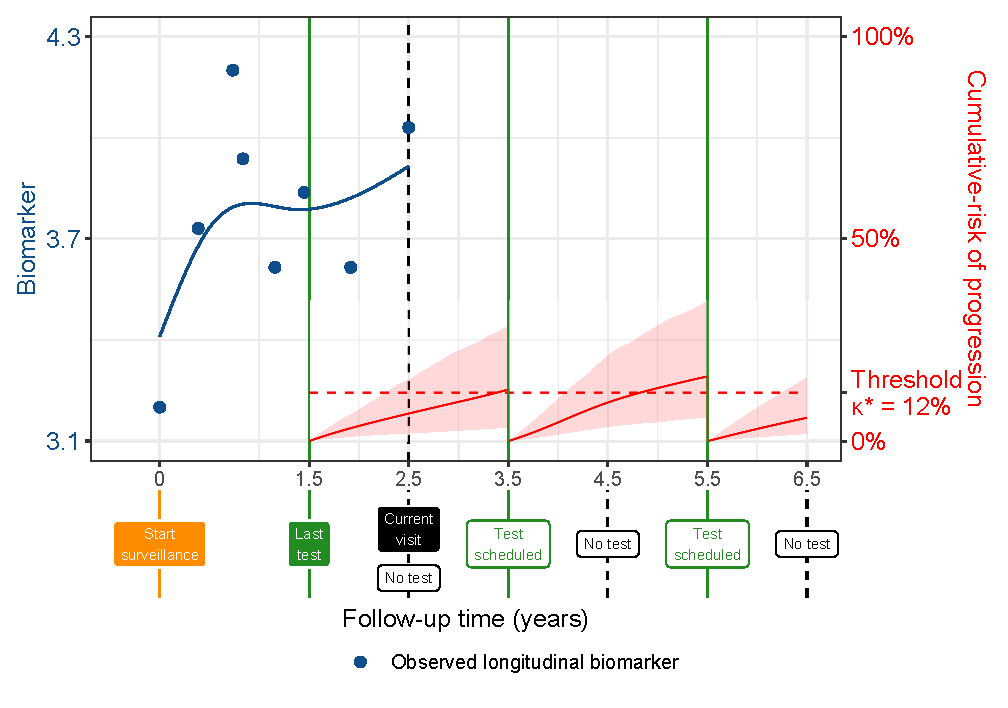
\includegraphics{images/schedule_explanation_102.eps}}
\caption{\textbf{Personalized Invasive Test Schedule Using Patient-specific Conditional Cumulative-risk of Progression}.  A single longitudinal outcome, namely, a continuous biomarker (observed: blue dots, fitted: blue line) of disease progression is used for illustration. The last test on which progression was not observed was conducted at $t=1.5$ years. The current visit time of the patient is $v=2.5$ years. Decisions for invasive test need to be made at a gap of every one year starting from the current visit until a horizon of 6.5 years. That is, $U=\{2.5, 3.5, 4.5, 5.5, 6.5\}$ years. Based on an example risk threshold of 12\% ($\kappa=0.12$) the future test decisions at time points in $U$ lead to a personalized schedule $S_j^{\kappa} (U \mid t=1.5, v=2.5) = \{3.5, 5.5\}$ years. The conditional cumulative-risk profiles $R_j(u_l \mid t_l, v)$ employed in~(\ref{eq:personalized_decision_grid}) are shown with red line (confidence interval shaded). It is called `conditional' because, for example, the second test at future time 5.5 years, is scheduled after accounting for the possibility that progression (true time $T^*_j$) may not have occurred until the time of the previously scheduled test at time $T^*_j>3.5$ years. All values are illustrative.} 
\label{fig:schedule_explanation}
\end{figure}

If patient $j$ never progressed in the period $[t, u_L]$, as we initially supposed, all $N_j$ tests in $\{s_1, \ldots, s_{N_j}\}$ will be conducted. However, fewer tests will be performed if the patient did progress at some point $T_j^* < u_L$. We formally define the discrete random variable denoting the number of performed tests in conjunction with the true progression time $T_j^*$ as:
\[
\mathcal N_j (S^\kappa_j) = \left \{
\begin{array}{ll}
1, & \mbox{ if } \; t < T^*_j \leq s_1,\\
2, & \mbox{ if } \; s_1 < T^*_j \leq s_2,\\
\vdots&\\
N_j, & \mbox{ if } \; s_{N_j-1} < T^*_j \leq s_{N_j},
\end{array}
\right.
\]
where $S^\kappa_j = \{s_1, \ldots, s_{N_j}\}$. The expected number of future tests for patient $j$ will be the expected value $E \big \{\mathcal N_j(S^\kappa_j)\big\}$. It is defined as:
\begin{equation*}
\label{eq:exp_tests}
E \big \{\mathcal N_j(S^\kappa_j)\big\} = \sum_{n = 1}^{N_j} n \times \mbox{Pr}(s_{n-1} < T^*_j \leq s_n \mid T^*_j \leq s_{N_j}), \quad s_0 = t,
\end{equation*}
where 
\begin{equation*}
\mbox{Pr}(s_{n-1} < T^*_j \leq s_n \mid T^*_j \leq s_{N_j}) = \frac{R_j(s_n \mid t, v) - R_j(s_{n-1} \mid t, v)}{R_j(s_{N_j} \mid t, v)}.
\end{equation*}

Similarly, we can define the expected time delay in detecting progression, under the assumption that progression occurs before $u_L$. Specifically, the random variable time delay is equal to the difference between the time of the test at which progression is observed and the true time of progression $T_j^*$, and is given by:
\[
\mathcal D_j (S^\kappa_j) = \left \{
\begin{array}{ll}
s_1 - T_j^*, & \mbox{ if } \; t < T^*_j \leq s_1,\\
s_2 - T_j^*, & \mbox{ if } \; s_1 < T^*_j \leq s_2,\\
\vdots&\\
s_{N_j} - T_j^*, & \mbox{ if } \; s_{N_j-1} < T^*_j \leq s_{N_j},
\end{array}
\right.
\]
The expected delay will be the expected value of $\mathcal D_j (S^\kappa_j)$ given by the expression:
\begin{equation*}
\label{eq:exp_delay}
E \big \{ \mathcal D_j(S^\kappa_j)\big\} = \sum_{n = 1}^{N_j} \Big\{s_n - E(T^*_j \mid s_{n-1}, s_n, v)\Big\} \times \mbox{Pr}(s_{n-1} < T^*_j \leq s_n\mid T^*_j \leq s_N),
\end{equation*}
where $E(T^*_j \mid s_{n-1}, s_n, v)$ denotes the conditional expected time of progression for the scenario $s_{n-1} < T^*_j \leq s_n$ and is calculated as the area under the corresponding survival curve:
\begin{equation*}
E(T^*_j \mid s_{n-1}, s_n, v) = s_{n-1} + \int_{s_{n-1}}^{s_n} \mbox{Pr}\Big\{T^*_j \geq u \mid s_{n-1} < T^*_j \leq s_n, \mathcal{Y}_{1j}(v), \ldots, \mathcal{Y}_{Kj}(v), \mathcal{A}_n\Big\} \mathrm{d}u,
\end{equation*}

The personalized schedule in~(\ref{eq:personalized_schedule_grid}), and the corresponding personalized expected number of tests and time delay, all have the advantage of getting updated with newly collected data over follow-up. Also, expected number of tests and time delay can be calculated for any schedule, fixed or personalized. Hence, patients/doctors can use them to compare different schedules. Although, a fair comparison of time delays between different schedules for the same patient, requires a compulsory test at a common horizon time point in all schedules.

\subsection{How to Select the Risk Threshold $\kappa$}
The risk threshold $\kappa$ controls the timing and the total number of invasive tests in the personalized schedule $S^\kappa_j$. Also, through the timing and total number of planned tests, $\kappa$ also indirectly affects the time delay (Figure~\ref{fig:delay_explanation}) that may occur in detecting progression if a particular schedule is followed. Hence, $\kappa$ should be chosen while balancing both the number of invasive tests (burden) and the time delay in detecting progression (shorter is beneficial).

To facilitate the choice of $\kappa$ in practice, and in accordance to our developments in the previous section, we translate different choices for this parameter into the expected number of test and time delay. More specifically, for a specific patient $j$ and at the current visit time $v$, we can construct the bi-dimensional Euclidean space of the expected total number of tests (x-axis) and time delay in detecting progression (y-axis) for test schedules planned by varying $\kappa$ in $[0, 1]$. An example of such a space is given in Figure~\ref{fig:kappa_choice}.
\begin{figure}
\centerline{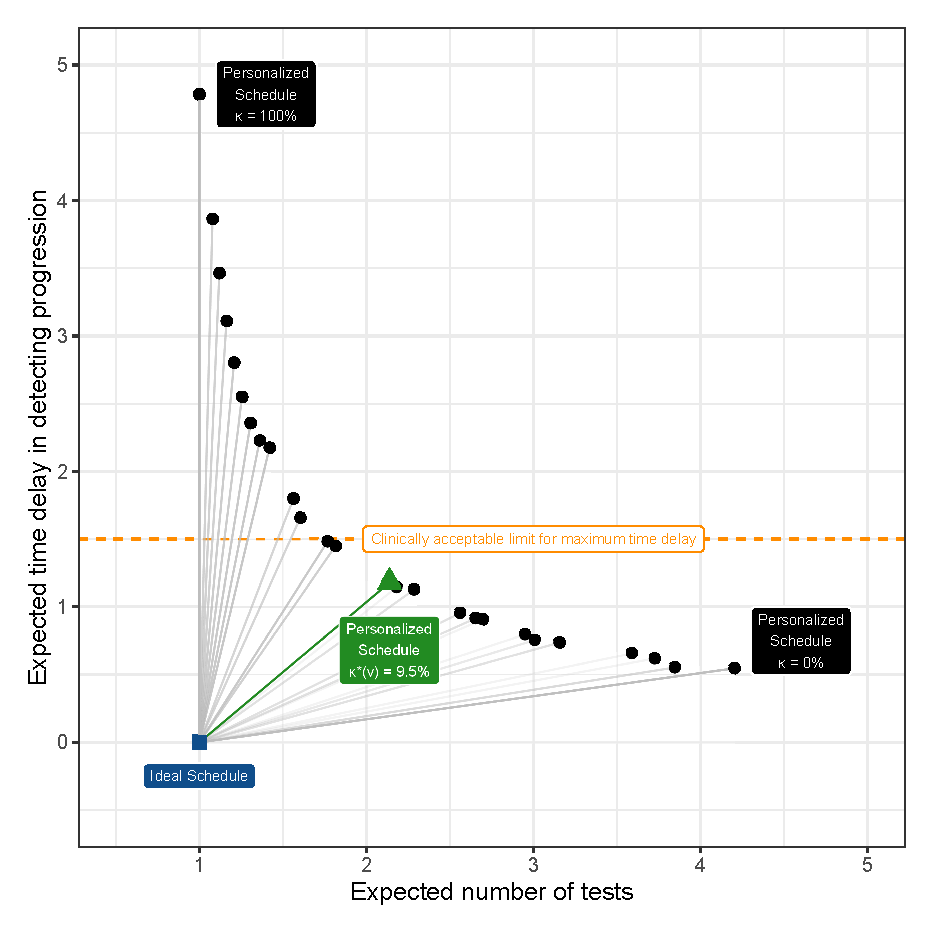
\includegraphics{images/kappa_choice_102.eps}}
\caption{\textbf{Automatic choice of risk threshold $0 \leq \kappa \leq 1$ using~(\ref{eq:kappa_choice})}. The ideal schedule of tests at point (1,0) is shown as a blue square. It plans exactly one invasive test at the true time of progression $T^*_j$ of a patient and hence leads to a zero time delay in detecting progression. Personalized schedules based on a grid of thresholds chosen between $0 \leq \kappa \leq 1$ are shown with black circles. Higher thresholds lead to fewer tests, but also higher expected time delay. We propose to choose the personalized schedule based on $\kappa^*(v)=9.5\%$ threshold (green triangle). This is because it has the least Euclidean distance (shown with a green line) to the ideal schedule. It is also possible to find the least distance under a certain clinically acceptable limit on time delay (orange dashed line), or number of tests.}
\label{fig:kappa_choice}
\end{figure}
The ideal schedule for $j$-th patient is the one in which only one test is conducted, at exactly the true time of progression $T^*_j$. In other words, the time delay will be zero. If we weigh the expected number of tests and time delay as equally important, then a current visit time specific risk threshold $\kappa^*(v)$ can be chosen as the threshold that minimizes Euclidean distance between the ideal schedule, i.e., point (1, 0) and the set of points representing the different personalized schedules $S^{\kappa}_j$ corresponding to various $\kappa \in [0, 1]$, i.e.,
\begin{equation}
\label{eq:kappa_choice}
\kappa^*(v) = \argmin_{0 \leq \kappa \leq 1} \sqrt{\Big[E\big\{\mathcal N_j(S^\kappa_j)\big\} - 1\Big]^2 + \Big[E\big\{\mathcal D_j(S^\kappa )\big\} - 0\Big]^2}.
\end{equation}
Additional clinical consequences of following a particular schedule, such as (quality-adjusted) life-years saved, can also be accommodated in~(\ref{eq:kappa_choice}). This requires first setting a point of optimality in a higher dimensional Euclidean space of such consequences, and then minimizing the Euclidean distance relative to this point of optimality.

An alternative approach is to constrain one of the two dimensions. For example, patients/doctors may not agree to more than a maximum number of planned future tests. They may also be apprehensive about having an expected time delay higher than a certain number of months. In such situations, the Euclidean distance in~(\ref{eq:kappa_choice}) can be minimized under constraints on the expected number of tests and/or expected time delay (Figure~\ref{fig:kappa_choice}). An additional benefit of this approach is that it alleviates the issue of time delay and number of tests having different units of measurement~\cite{cook1994equivalence}.

